\documentclass[journal,12pt,onecolumn]{IEEEtran}
\usepackage{cite}
\usepackage{caption}
\usepackage{graphicx}
\usepackage{amsmath,amssymb,amsfonts,amsthm}
\usepackage{algorithmic}
\usepackage{graphicx}
\usepackage{textcomp}
\usepackage{xcolor}
\usepackage{txfonts}
\usepackage{listings}
\usepackage{enumitem}
\usepackage{mathtools}
\usepackage{gensymb}
\usepackage{comment}
\usepackage[breaklinks=true]{hyperref}
\usepackage{tkz-euclide} 
\usepackage{listings}
\usepackage{gvv}
%\def\inputGnumericTable{}
\usepackage[latin1]{inputenc} 
\usetikzlibrary{arrows.meta, positioning}
\usepackage{xparse}
\usepackage{color}                                            
\usepackage{array}                                            
\usepackage{longtable}                                       
\usepackage{calc}                                             
\usepackage{multirow}
\usepackage{multicol}
\usepackage{hhline}                                           
\usepackage{ifthen}                                           
\usepackage{lscape}
\usepackage{tabularx}
\usepackage{array}
\usepackage{float}

\usepackage{float}
%\newcommand{\define}{\stackrel{\triangle}{=}}
\theoremstyle{remark}
\usepackage{circuitikz}
\captionsetup{justification=centering}
\usepackage{tikz}

\title{Matrices in Geometry 5.2.40}
\author{EE25BTECH11037 - Divyansh}
\begin{document}
\vspace{3cm}
\maketitle
{\let\newpage\relax\maketitle}
\textbf{Question: }
Solve
\begin{align*}
    \frac{4}{x}+3y=14 \\
    \frac{3}{x} -4y =23
\end{align*}

\vspace{2mm}

\textbf{Solution:}
\vspace{1mm}
We have the following two equations as:
\begin{align}
    \myvec{4 & 3 \\ 3 & -4}\myvec{\frac{1}{x} \\ y}=\myvec{14 \\ 23}
\end{align}
Writing the augmented matrix for these equations,
\begin{align}
    \myvec{4 & 3 & \vrule & 14 \\ 3 & -4 & \vrule & 23} \overset{R_1 \rightarrow R_1 /4}{\longleftrightarrow} \myvec{1 & 3/4 & \vrule & 7/2 \\ 3 & -4 & \vrule & 23}\overset{R_2 \rightarrow R_2-3R_1}{\longleftrightarrow} \myvec{1 & 3/4 & \vrule & 7/2 \\ 0 & -25/4 & \vrule & 25/2} \overset{R_2 \rightarrow \frac{-4}{25}R_2}{\longleftrightarrow}\\
    \myvec{1 & 3/4 & \vrule & 7/2 \\ 0 & 1 & \vrule & -2}\overset{R_1 \rightarrow R_1-\frac{3}{4} R_2}{\longleftrightarrow} \myvec{1 & 0 & \vrule & 5 \\ 0 & 1 & \vrule & -2}
\end{align}
This implies that
\begin{align}
    \myvec{\frac{1}{x} \\ y} = \myvec{5 \\ -2}\implies x=\dfrac{1}{5} \ , \ y=-2
\end{align}
\begin{figure}[H]
    \centering
    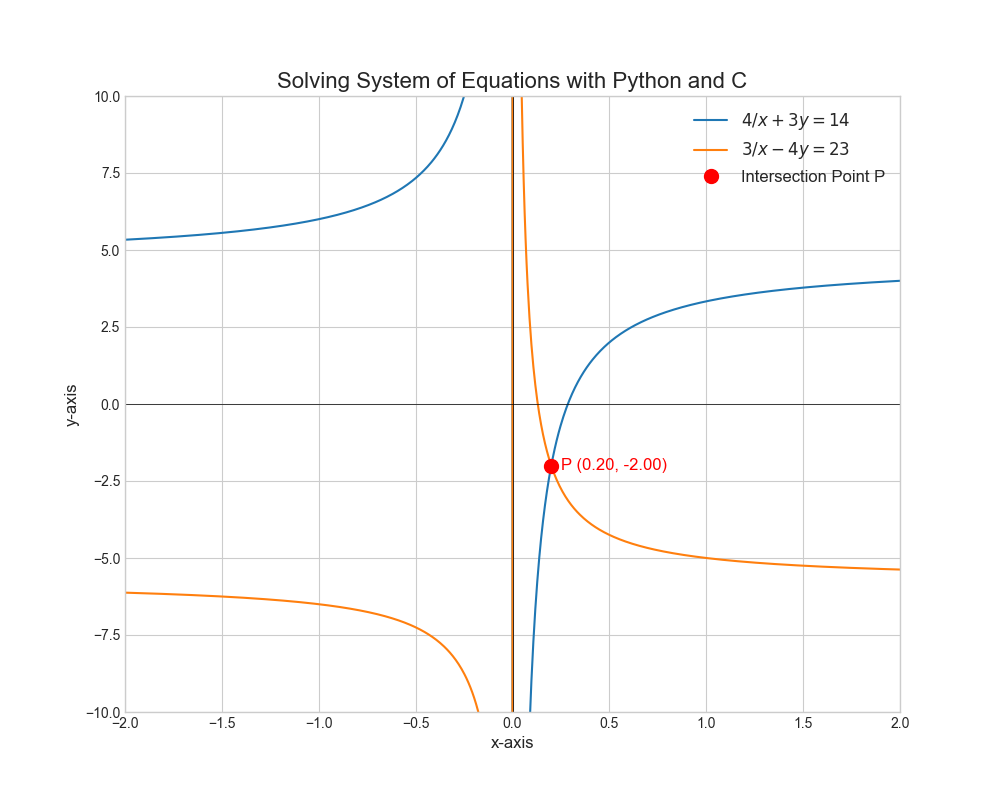
\includegraphics[width=1\columnwidth]{figs/1.png}
    \caption{Graph for 5.2.40}
    \label{fig:placeholder}
\end{figure}
\end{document}